\documentclass[11pt]{article}
\usepackage{fullpage}
\usepackage{amsthm}
\usepackage{amsmath} \usepackage{amssymb}
\usepackage{graphicx}

\graphicspath{ {./imgs/} }

\setlength{\parindent}{0pt}

\title{Distributed Algorithms (CO347)}
\author{Michael Tsang}

\newtheorem{defn}{Definition}
\newtheorem{eg}{Example}
\newtheorem{theo}{Theorem}
\newtheorem{lem}{Lemma}

\begin{document}

\maketitle
\section{Motivation}
\subsection{Why a Distributed System?}
\begin{itemize}
  \item Computation and data distribution.
  \item Performance through parallelisation and distribution.
  \item Reliability and availability through replication, fault-tolerance, security.
  \item Scalability, modularity, evolvability.
  \item Heterogenity of hardware and software.
\end{itemize}

\subsection{What is a Distributed System?}
\begin{itemize}
  \item A set of processes connected by a network.
    \begin{itemize}
      \item Machines can be located across the planet.
      \item Communicate via message passing, no shared memory.
    \end{itemize}
  \item No common physical clock.
    \begin{itemize}
      \item No total order on events by time.
    \end{itemize}
\end{itemize}

\subsection{Assumptions}
When designing distributed systems, we have to consider different assumptions.

\subsubsection{Timing}
\begin{itemize}
  \item \textbf{Synchronous systems}:
    \begin{itemize}
      \item Upper bound on process delays.
      \item Upper bound on time for a message to be delivered.
      \item Can translate results to asynchronous models.
    \end{itemize}
  \item \textbf{Asynchronous systems}:
    \begin{itemize}
      \item Processes and communication take arbitrary time.
      \item No assumption that processes have physical clocks, but can be useful to use logical clocks.
    \end{itemize}
  \item \textbf{Partially synchronous systems}:
    \begin{itemize}
      \item Real-world systems are mostly synchronous with asynchronous periods.
      \item Assume the system is eventutally synchronous.
    \end{itemize}
\end{itemize}

\subsubsection{Failures}
\begin{itemize}
  \item \textbf{No failures}:
    \begin{itemize}
      \item Unrealistic.
    \end{itemize}
  \item \textbf{Process failure}:
    \begin{itemize}
      \item e.g.\ software bugs; OS/user termination; OS failure.
      \item Process stops sending messages it is supposed to send.
      \item Process sends messages it is not supposed to send.
    \end{itemize}
  \item \textbf{Link failure}:
    \begin{itemize}
      \item e.g.\ cable, router, wireless, adversary.
      \item Inter-process communication failure, e.g.\ non-delivery of messages; corrupt messages; duplicates.
      \item Need for reliable protocols and secure channels.
      \item Partitioned networks.
    \end{itemize}
\end{itemize}

\subsubsection{Failure Classes}
\begin{itemize}
  \item \textbf{Process crash failure} (crash-stop failure):
    \begin{itemize}
      \item Process halts and does not perform further action.
      \item Different types:
        \begin{itemize}
          \item \textbf{Fail-stop} - can be reliably detected by other processes.
          \item \textbf{Fail-silent} - cannot be reliably detected.
          \item \textbf{Fail-noisy} - detection takes time.
          \item \textbf{Fail-recovery} - crashed processes can recover
        \end{itemize}
      \item Non-faulty processes are a \textbf{correct process}.
    \end{itemize}
  \item \textbf{Link failure}:
    \begin{itemize}
      \item Link goes down and stays down.
      \item Network may partition or remain connected.
    \end{itemize}
  \item \textbf{Omission failure}:
    \begin{itemize}
      \item Two types:
        \begin{itemize}
          \item \textbf{Send omission} - does not send all required messages.
          \item \textbf{Receive omission} - does not receive all require messages.
        \end{itemize}
    \end{itemize}
  \item \textbf{Byzantine failure} (fail-arbitrary):
    \begin{itemize}
      \item Arbitrary (or malicious) behaviour.
    \end{itemize}
\end{itemize}

\subsubsection{Communication}
\begin{itemize}
  \item \textbf{Asynchronous message passing}:
    \begin{itemize}
      \item The process sending a message continues after sending.
      \item We can build a \textbf{synchronous message passing} mechanism, e.g.\ process waits until message is delivered to the receiving process.
      \item We can build a \textbf{shared memory abstraction}.
    \end{itemize}
  \item \textbf{Reliable message communication}:
    \begin{itemize}
      \item Assume that messages sent using reliable protocol.
      \item Communications can still fail.
      \item Use TCP to send messages, simulate network failure by dropping messages in software.
    \end{itemize}
  \item \textbf{Message delays are bounded}:
    \begin{itemize}
      \item Processes timeout if message is delayed too long.
    \end{itemize}
\end{itemize}

\section{Reliable Broadcast}
We discuss algorithms for reliable broadcast in \textbf{asynchronous message-passing} distributed systems that are subject to \textbf{process failure}, we want:
\begin{itemize}
  \item To guarantee that messages are consistently delivered to processes.
  \item Agreement on delivered messages.
  \item No ordering among delivered messages.
\end{itemize}

\subsection{Structure}
Each distributed process is a set of interconnected components.
Each distributed process will typically have the same set of components.

\begin{figure}[htb!]
  \centering
  \caption{Elixir mappings.}
  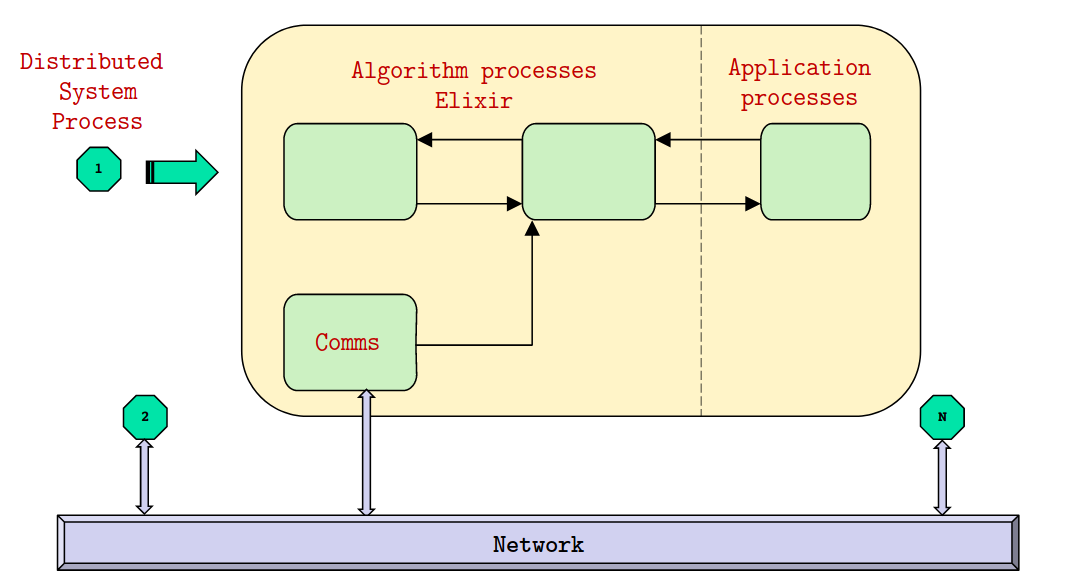
\includegraphics[scale=0.3]{elixirmapping}
\end{figure}

We implement this in \textit{Elixir} where a distributed system process is 1 \textit{Elixir} node, which is many \textit{Elixir} processes.
The components are \textit{Elixir} processes which use message passing for intra-node interactions

\subsection{Assumptions}
\begin{itemize}
  \item \textbf{Asynchronous system}:
    \begin{itemize}
      \item No bound on message delays.
      \item No bound on time to execute a local process step.
      \item Time to execute a step is finite.
    \end{itemize}
  \item Processes interact by \textbf{message passing}.
  \item \textbf{Message passing is reliable}.
  \item Every process can logically communicate with every other.
  \item Number of processes fixed and known.
  \item Crashed processes do not continue.
\end{itemize}

\subsection{Classes of Broadcast}
\begin{itemize}
  \item \textbf{One shot} - each message is considered separately from others:
    \begin{itemize}
      \item Best-Effort Broadcast (BEB).
      \item Reliable Broadcast (RB).
      \item Uniform Reliable Broadcast (URB).
    \end{itemize}
  \item \textbf{Multishot} - involve all messages that are broadcast:
    \begin{itemize}
      \item FIFO Message delivery.
      \item Casual Order Message Delivery.
      \item Total Order Message Delivery.
    \end{itemize}
\end{itemize}

\subsection{Perfect Point-to-Point Links (PL)}
The distributed processes communicate with PL components.
\begin{figure}[htb!]
  \centering
  \caption{Perfect point-to-point links component.}
  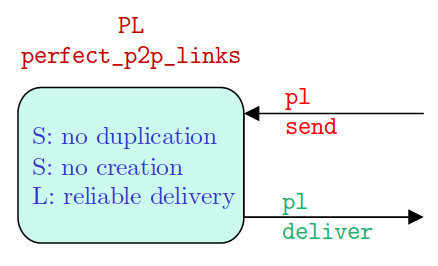
\includegraphics[scale=0.3]{pl}
\end{figure}

\begin{itemize}
  \item \textbf{Reliable Delivery (L)} - if Alice and Bob are correct processes, then every message sent by Alice to Bob is eventually delivered to Bob.
  \item \textbf{No Duplication (S)} - no message is delivered to a process more than once.
  \item \textbf{No Creation (S)} - no message is delivered unless it was sent.
\end{itemize}

\subsection{Best-Effort Broadcast (BEB)}
Given a list of all processes and a message, we send the message to all processes (including ourselves) with multiple sends:
\begin{itemize}
  \item If sending is reliable, then every correct process will receive a copy, crashed processes may or may not have received a copy.
  \item The messages will be received at arbitrary times.
  \item If the sending process crashes during broadcast, some arbitrary subset of processes will receive the message.
  \item The sender does not know which processes have received the message.
\end{itemize}

\begin{figure}[htb!]
  \centering
  \caption{Best-effort broadcast component.}
  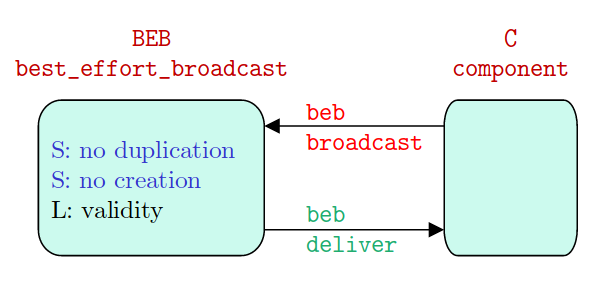
\includegraphics[scale=0.3]{beb}
\end{figure}

We assume messages are unique (e.g.\ they include a process-id and seq-no), no process broadcasts a message twice, and no two processes every broadcast the same message.

\begin{itemize}
  \item \textbf{Validity (L)} - if a correct process broadcasts a message, then every correct process eventually delivers it.
  \item \textbf{No Duplication (S)} - no message is delivered to a process more than once.
  \item \textbf{No Creation (S)} - no message is delivered unless it was broadcast.
\end{itemize}

\subsubsection{BEB Basic Broadcast}
\begin{figure}[htb!]
  \centering
  \caption{Basic broadcast.}
  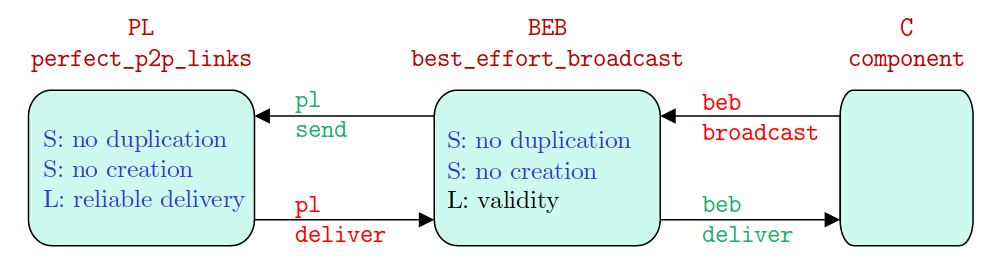
\includegraphics[scale=0.3]{bebpl}
\end{figure}

\begin{itemize}
  \item BEB sends a message to each process using the PL component - this works as PL ensures all correct processes deliver messages, as long as the sender does not crash.
  \item BEB is fail-silent.
  \item $1$ broadcast step and $O(N)$ messages, where $N$ is the number of processes.
  \item BEB derives its S\&L properties from PL.
\end{itemize}

\begin{itemize}
  \item \textbf{No Duplication (S)} and \textbf{No Creation (S)} dervied from PL.
  \item \textbf{No Duplication (S)} also assumes messages are unique.
  \item \textbf{Validity (L)} derived from \textbf{Reliable Delivery (L)} in PL and the fact that the message needs to be sent to all processes.
\end{itemize}

\begin{figure}[htb!]
  \centering
  \caption{BEB code.}
  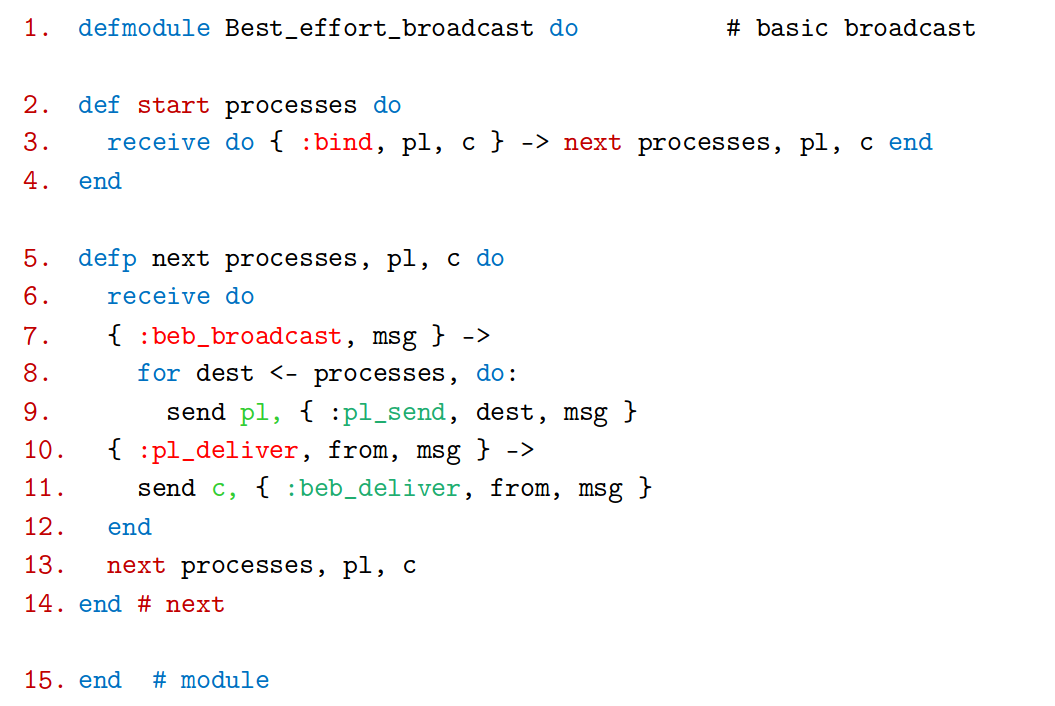
\includegraphics[scale=0.3]{bebcode}
\end{figure}

\subsection{Reliable Broadcast (RB)}
\begin{figure}[htb!]
  \centering
  \caption{Reliable broadcast component.}
  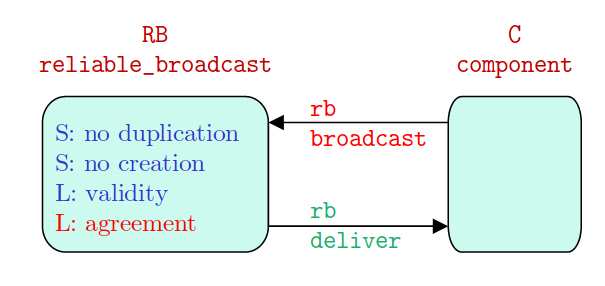
\includegraphics[scale=0.3]{rb}
\end{figure}
All correct processes will agree on the messages they deliver, even if the broadcasting process crashes while sending.

\begin{itemize}
  \item \textbf{Validity (L)}, \textbf{No Duplication (S)}, and \textbf{No Creation (S)} as in BEB.
  \item \textbf{Agreement (L)}:
    \begin{itemize}
      \item If a correct process delivers message $M$, then every correct process also delivers $M$.
      \item Validity and Agreement together provide a \textbf{Termination} property for broadcasting a message.
      \item Faulty process could deliver messages not delivered by correct processes.
    \end{itemize}
\end{itemize}

\subsubsection{Eager RB (fail-silent)}
\begin{figure}[htb!]
  \centering
  \caption{Eager RB.}
  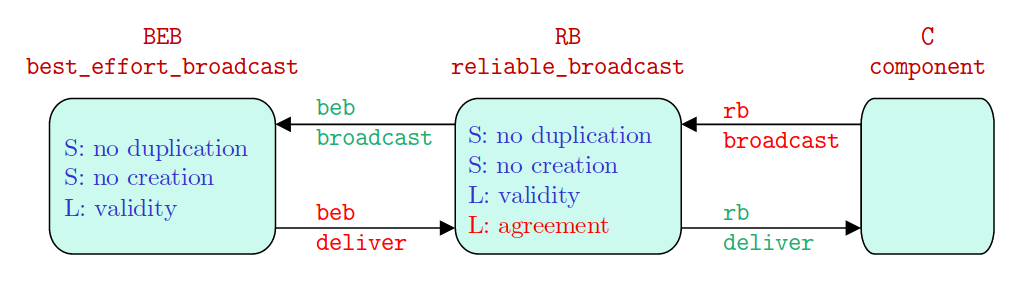
\includegraphics[scale=0.3]{rbbeb}
\end{figure}

Every process re-broadcasts every message it delivers.
If the broadcasting process crashes, then the message will be forwarded by other processes using BEB.

At best $1$ broadcast step, at worst $O(N)$ broadcast steps if processes crash in sequence.
$O(N^2)$ messages.

\begin{itemize}
  \item \textbf{No Creation (S)} and \textbf{Validity (L)} derived from BEB.
  \item \textbf{No Duplication (S)} as messages delivered are kept track of, and messages are assumed to be unique.
  \item \textbf{Agreement (L)} is derived from \textbf{Validity (L)} of BEB, and the fact that every correct process forwards every message it delivers.
\end{itemize}

\begin{figure}[htb!]
  \centering
  \caption{Eager RB code.}
  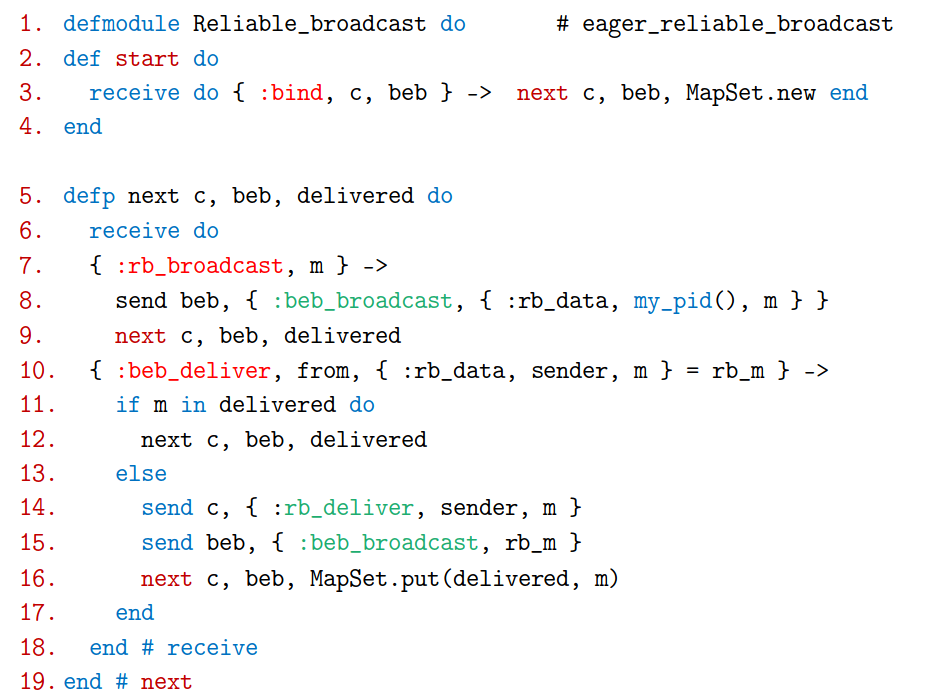
\includegraphics[scale=0.3]{eagercode}
\end{figure}

\subsubsection{Lazy RB (fail-stop)}
\begin{figure}[htb!]
  \centering
  \caption{Lazy RB.}
  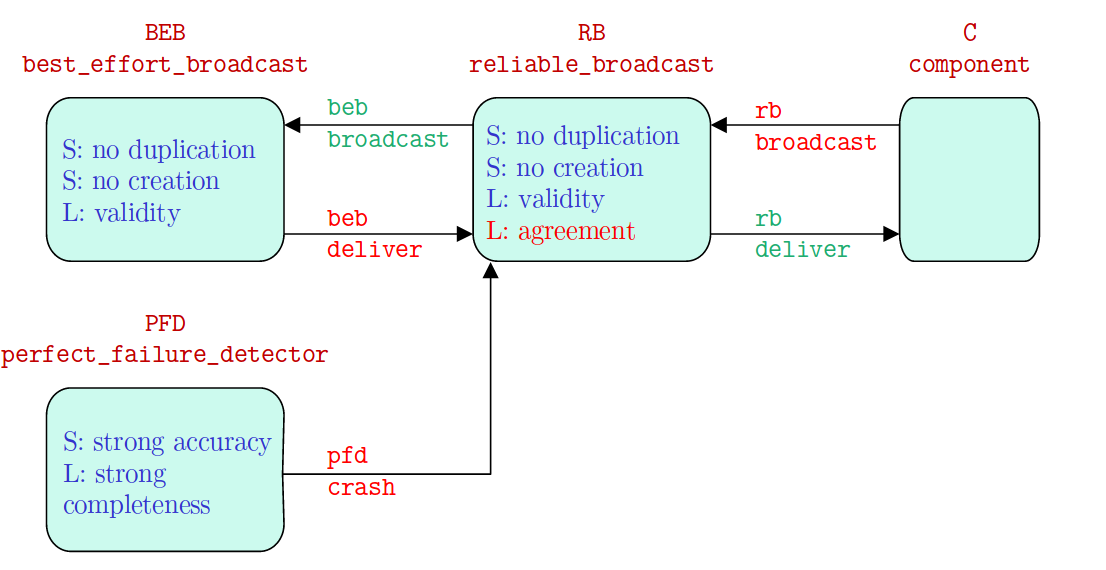
\includegraphics[scale=0.3]{lazyrb}
\end{figure}

Uses BEB, but includes a failure detector component to detect processes that have failed (and stopped).
When a crash is detected, all messages from that process are broadcast.
When a messsage is received from a crashed process then the message is broadcast, otherwise if it is a correct process it is not.

\begin{itemize}
  \item \textbf{Agreement (L)} is derived from the \textbf{Validity (L)} from BEB, that every correct process forwards every message it delivers when it detects a crashed process, and from PFD.
  \item Other properties follow as for the Eager RB.
\end{itemize}

\begin{figure}[htb!]
  \centering
  \caption{Lazy RB code, part 1.}
  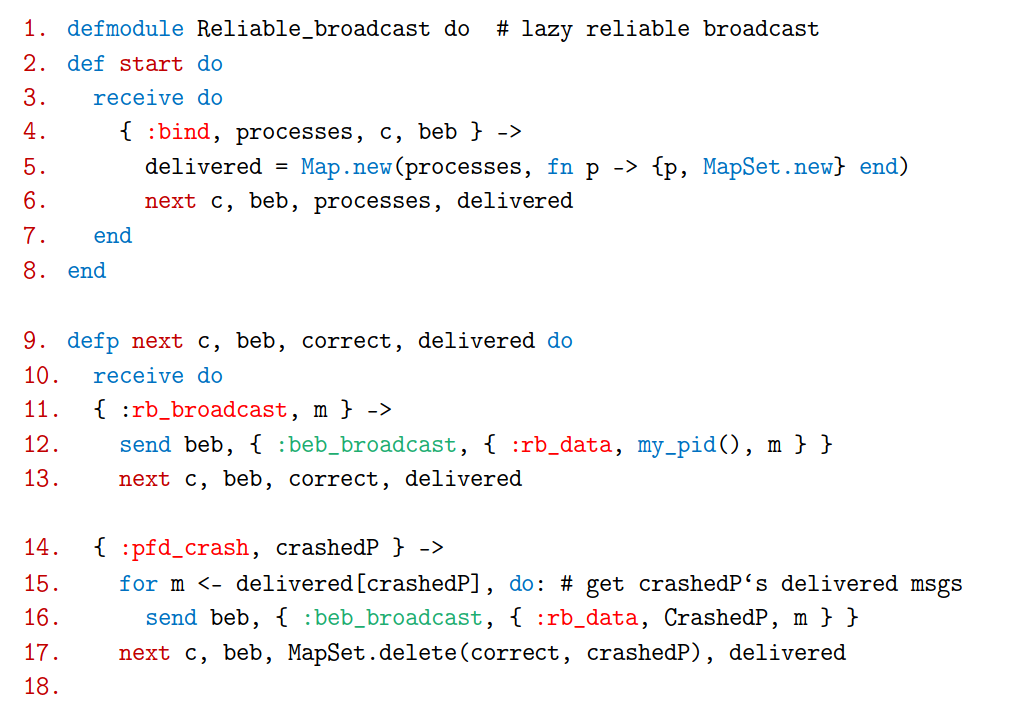
\includegraphics[scale=0.3]{lazycode1}
\end{figure}

\begin{figure}[htb!]
  \centering
  \caption{Lazy RB code, part 2.}
  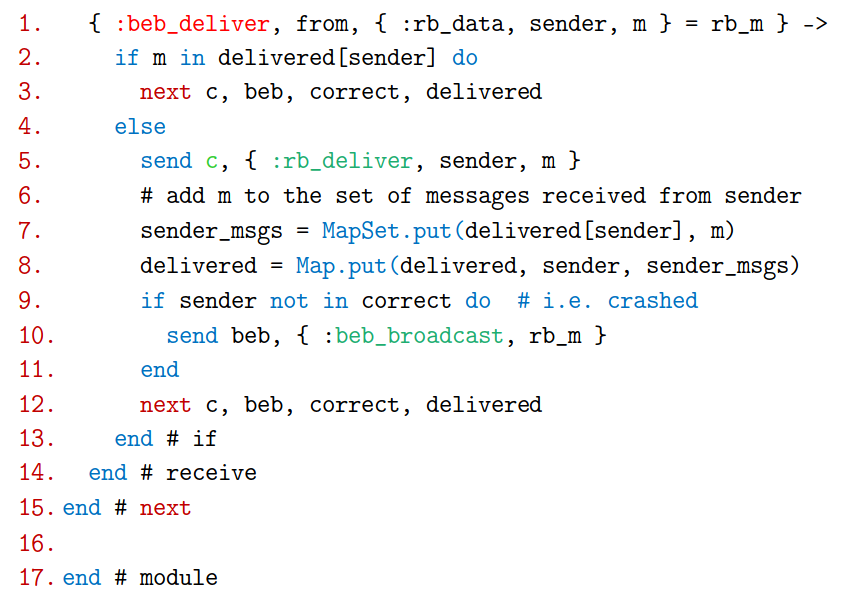
\includegraphics[scale=0.3]{lazycode2}
\end{figure}

\subsection{Failure Detectors}
\begin{itemize}
  \item \textbf{Perfect Failure Detector} $P$:
    \begin{itemize}
      \item Provides processes with a list of suspected (detected) processes that have crashed.
      \item Makes timing assumptions (assumes systems are not asynchronous).
      \item Never changes its view - suspects remain suspected forever.
    \end{itemize}
  \item \textbf{Eventually Perfect Failure Detector}: $\Diamond P$:
    \begin{itemize}
      \item May make mistakes but will eventually detect a crashed process.
    \end{itemize}
\end{itemize}

It has the following safety and liveness properties:
\begin{itemize}
  \item \textbf{Strong Completeness (L)} - every process that crashes will eventually be permanently suspected by every correct process.
  \item \textbf{Strong Accuracy (S)} - no process is suspected before it crashes.
  \item \textbf{Eventually Strong Accuracy (L)} - eventually no correct process is suspected.
\end{itemize}

\subsubsection{PFD Exclude on Timeout}
\begin{figure}[htb!]
  \centering
  \caption{Exclude on timeout.}
  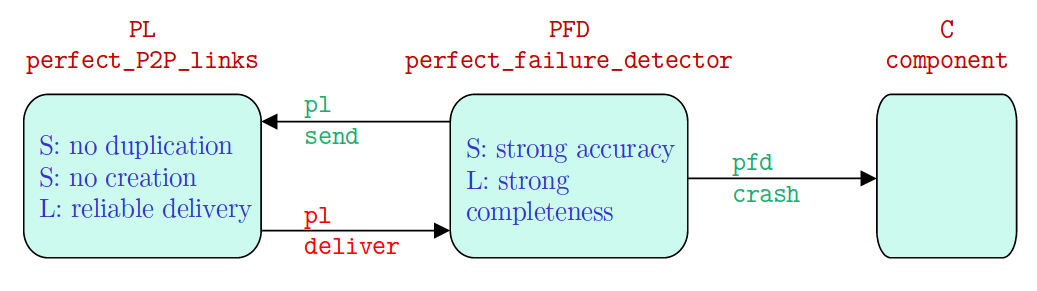
\includegraphics[scale=0.3]{pfd}
\end{figure}

Uses PL to exchange \textit{heartbeat} messages with a timeout mechanism.
The timeout delay must be large enough for all sends to processes, processing time, and replies back.
After timeout, processes from which a reply has not been received are considered crashed, even if it is alive and the reply arrived after timeout.

\begin{itemize}
  \item \textbf{Strong Completeness (L)}:
    \begin{itemize}
      \item If a process crashes, it stops replying to heartbeat messages; no process will deliver its reply.
      \item PL ensures no message is delivered unless sent.
      \item Then every correct process will detect the crash.
    \end{itemize}
  \item \textbf{Strong Accuracy (S)}:
    \begin{itemize}
      \item A process is suspected only if no reply is delivered before timeout.
    \end{itemize}
\end{itemize}

\begin{figure}[htb!]
  \centering
  \caption{PFD code, part 1.}
  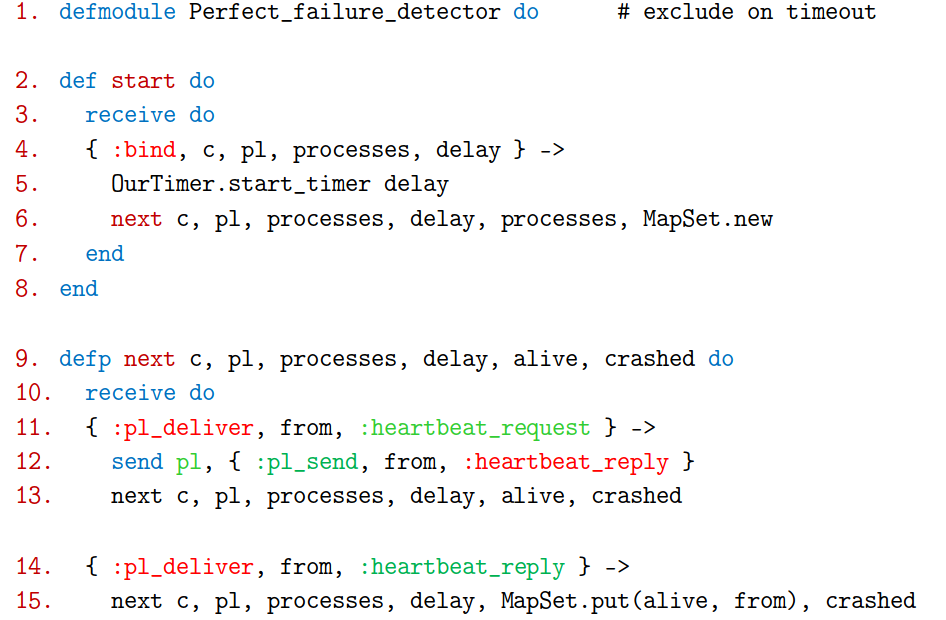
\includegraphics[scale=0.3]{pfdcode1}
\end{figure}

\begin{figure}[htb!]
  \centering
  \caption{PFD code, part 2.}
  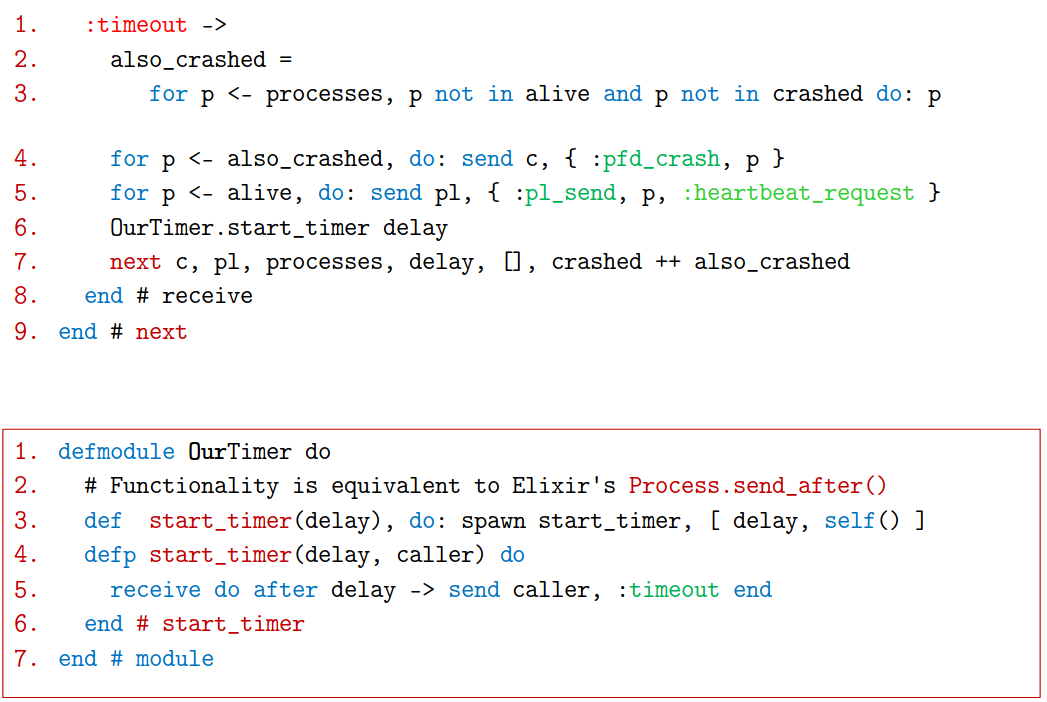
\includegraphics[scale=0.3]{pfdcode2}
\end{figure}


\subsection{Process Configuration}
Each distributed process is in the configuration seen in figure \ref{fig:processconf}.

\begin{figure}[htb!]
  \centering
  \caption{Full configuration of a distributed process.}
  \label{fig:processconf}
  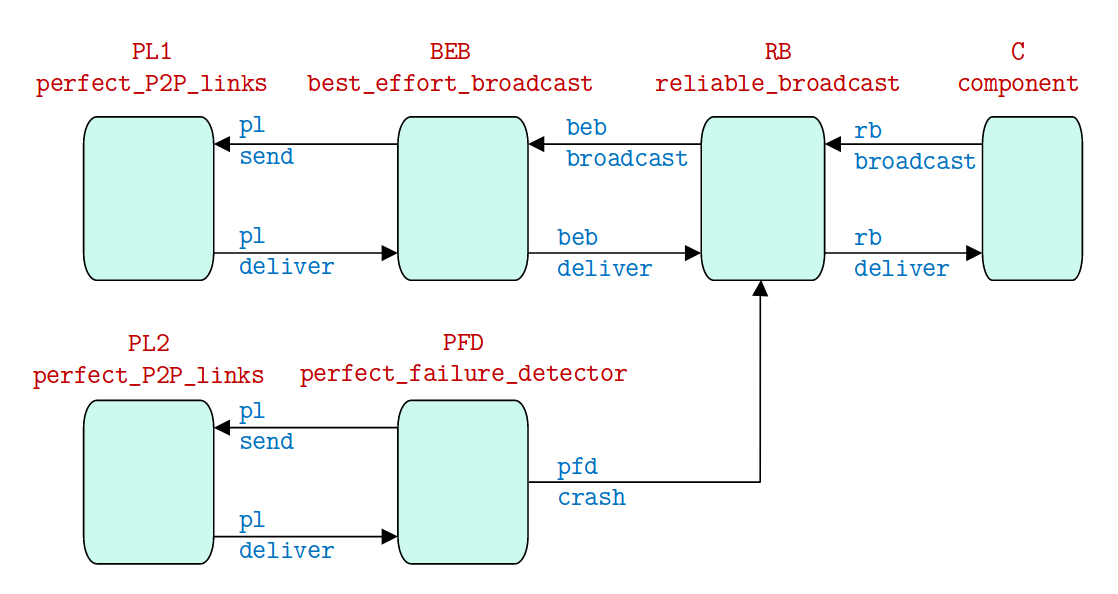
\includegraphics[scale=0.3]{processconf}
\end{figure}

\subsection{Uniform Reliable Broadcast (URB)}
\begin{figure}[htb!]
  \centering
  \caption{Uniform reliable broadcast.}
  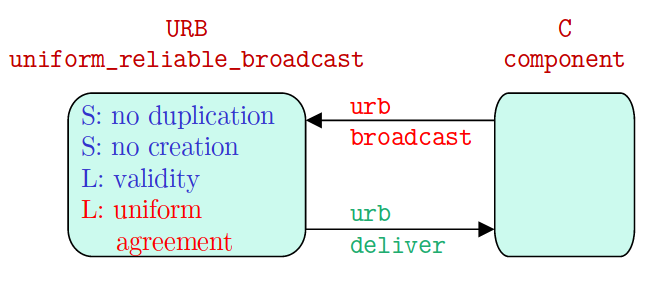
\includegraphics[scale=0.3]{urb}
\end{figure}

\begin{itemize}
  \item \textbf{Validity (L)}, \textbf{No Duplication (S)}, and \textbf{No Creation (S)} are the same as for BEB and RB.
  \item \textbf{Uniform Agreement (L)}:
    \begin{itemize}
      \item If a process (not necessarily correct) delivers a message $M$, then every correct process will also deliver $M$.
      \item The set of messages delivered by a faulty process is always a subset of messages delivered by a correct process.
      \item Use case may be to ensure consistency in financial transactions.
    \end{itemize}
\end{itemize}

\subsubsection{Majority-Ack URB}
\begin{figure}[htb!]
  \centering
  \caption{Majority-ack URB.}
  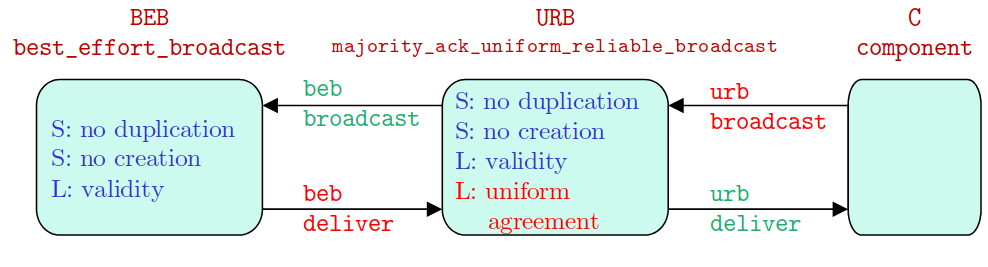
\includegraphics[scale=0.3]{majorityack}
\end{figure}

The message is only delivered after the message has been BEB-delivered by a majority (\textit{quorum}) of processes - at least one correct process is in the majority.

This is \textbf{fail-silent} as crashes are not detected, but it is \textbf{assumed the majority are correct processes}.

If process $P$ \texttt{beb\_deliver}s message $M$, then $P$ will eventually \texttt{urb\_deliver} M.
If $P$ \texttt{beb\_broadcast}s $M$, then all correct processes \texttt{beb\_broadcast} $M$.
Assuming the majority is correct, $P$ will eventually \texttt{beb\_deliver} $M$ from the majority of processes, then it will \texttt{urb\_deliver} $M$.
Then:
\begin{itemize}
  \item \textbf{No Creation (S)} follows from the corresponding safety property of BEB.
  \item \textbf{No Duplication (S)} as the algorithm keeps track of messages that have been \texttt{urb\_deliver}ed.
  \item \textbf{Validity (L)}:
    \begin{align*}
      P \texttt{ urb\_broadcast } M &\implies P \texttt{ beb\_broadcast } M \\
                                    &\implies P \texttt{ beb\_deliver } M \\
                                    &\implies P \texttt{ urb\_deliver } M
    \end{align*}
  \item \textbf{Uniform Agreement (L)}, if $Q$ is any process that \texttt{urb\_deliver}s $M$, then:
    \begin{itemize}
      \item $Q$ \texttt{beb\_deliver}ed $M$ from the majority of processes, and at least $1$ correct process \texttt{beb\_broadcast}ed $M$ (assumption).
      \item THen all correct processes eventually \texttt{beb\_deliver} $M$, and will also eventually \texttt{urb\_deliver} $M$.
    \end{itemize}
\end{itemize}

\begin{figure}[htb!]
  \centering
  \caption{Majority-ack URB code, part 1.}
  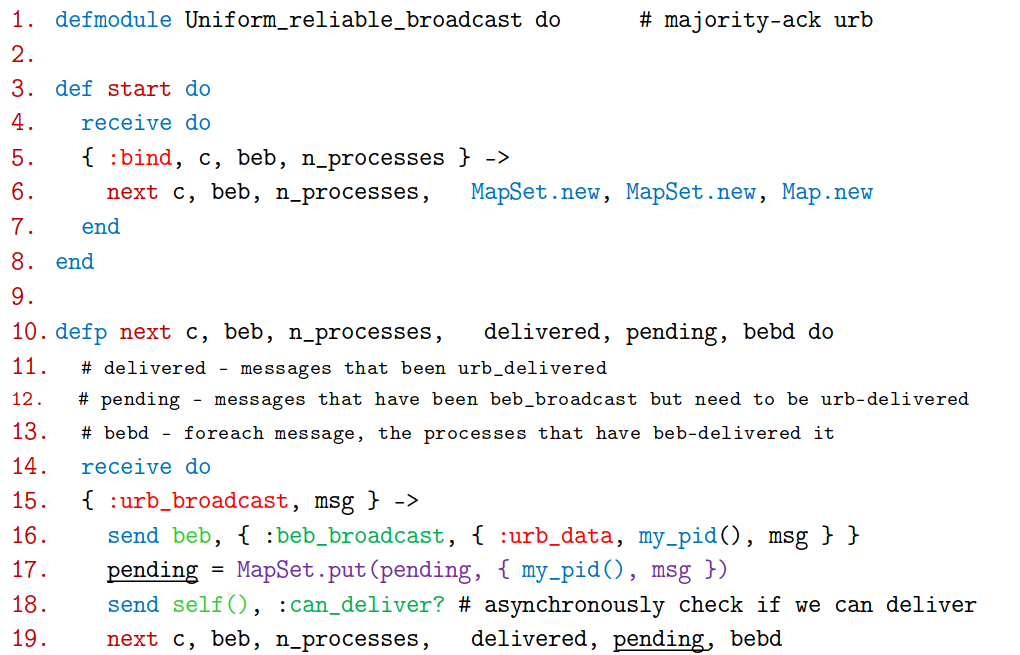
\includegraphics[scale=0.3]{urbcode1}
\end{figure}

\begin{figure}[htb!]
  \centering
  \caption{Majority-ack URB code, part 2.}
  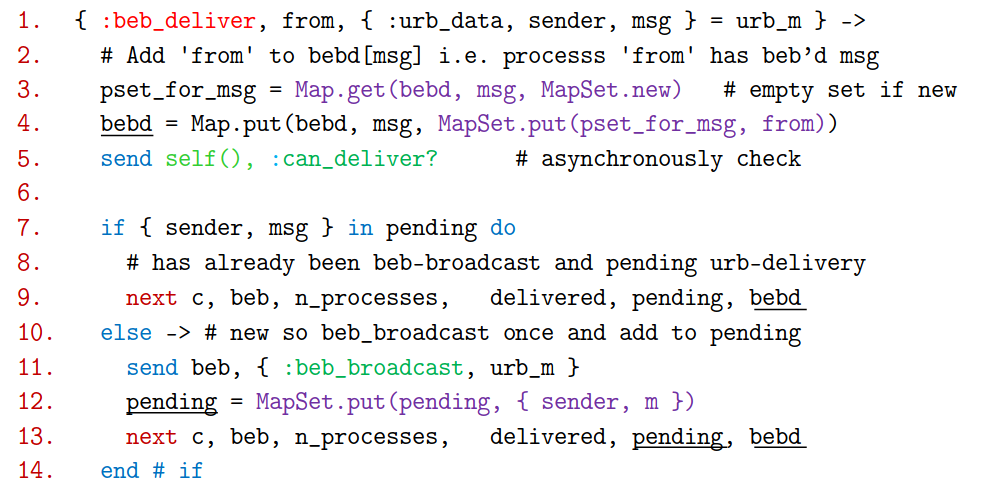
\includegraphics[scale=0.3]{urbcode2}
\end{figure}

\begin{figure}[htb!]
  \centering
  \caption{Majority-ack URB code, part 3.}
  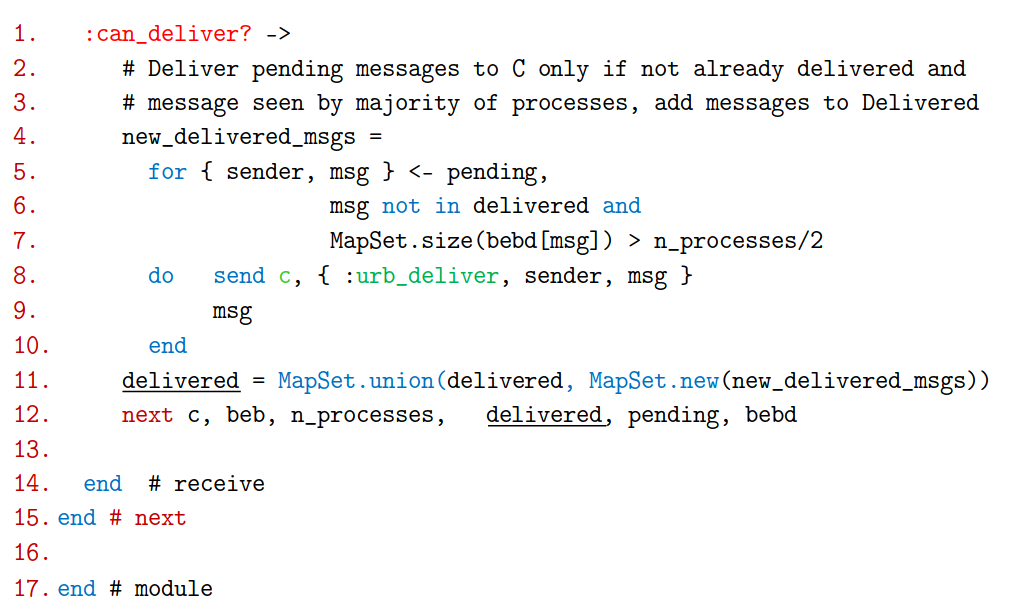
\includegraphics[scale=0.3]{urbcode3}
\end{figure}

\section{FIFO, Causal, and Total Order Broadcast}
\begin{itemize}
  \item \textbf{First In, First Out (FIFO)} - messages broadcast by a process are delivered in their broadcast order.
  \item \textbf{Causal Order (CO)} - messages broadcast by a process are delivered in their \textit{causal} order.
  \item \textbf{Total Order (TO)} - all correct processes deliver the same (global) sequence of messages, impossible in an asynchronous system.
\end{itemize}

\subsection{FIFO Regular RB (FRB)}
\begin{figure}[htb!]
  \centering
  \caption{FRB component.}
  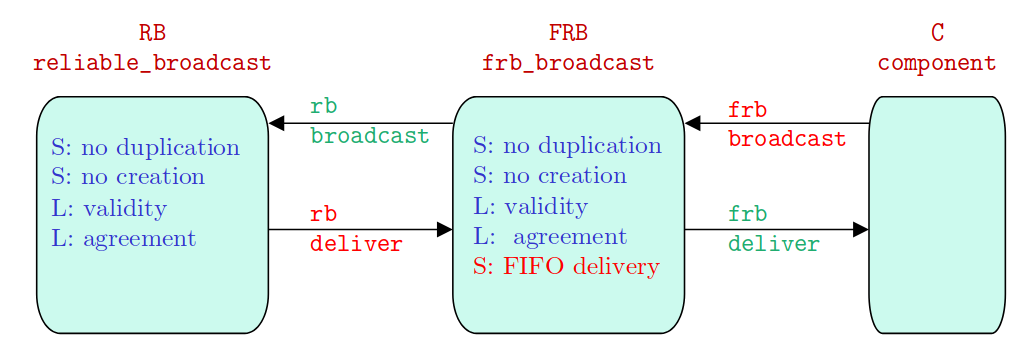
\includegraphics[scale=0.3]{fifo}
\end{figure}

FIFO regular reliable broadcast has the same reliability properties as RB, plus the ordering property that if a process broadcasts $M1$ before it broadcasts $M2$, then all \textbf{correct processes} will deliver $M1$ before $M2$.
This does not affect the messages of different senders.

\begin{figure}[htb!]
  \centering
  \caption{FRB code, part 1.}
  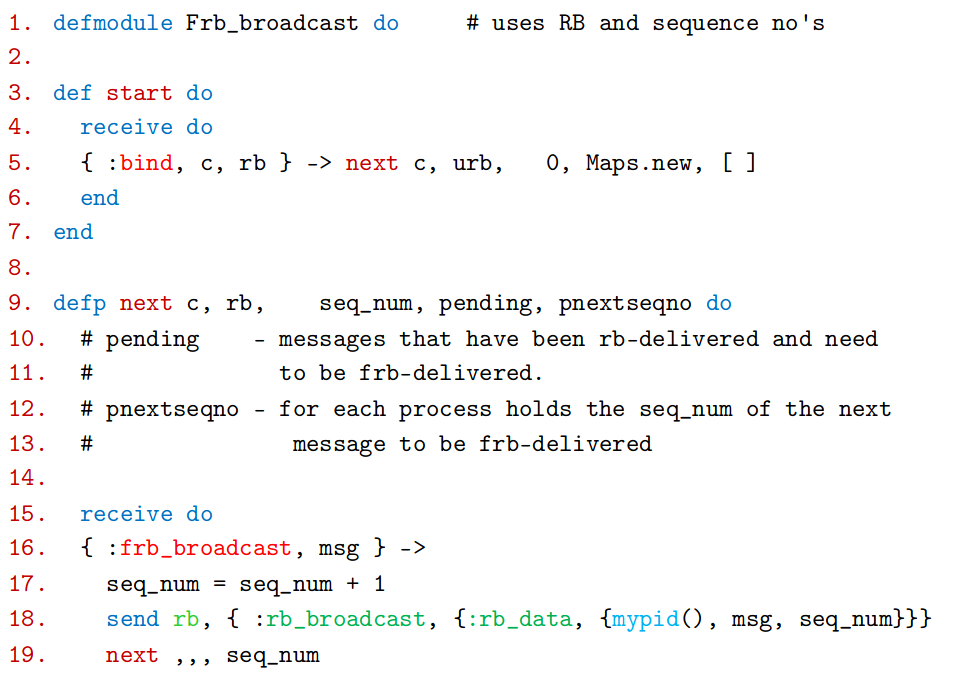
\includegraphics[scale=0.3]{frbcode1}
\end{figure}

\begin{figure}[htb!]
  \centering
  \caption{FRB code, part 2.}
  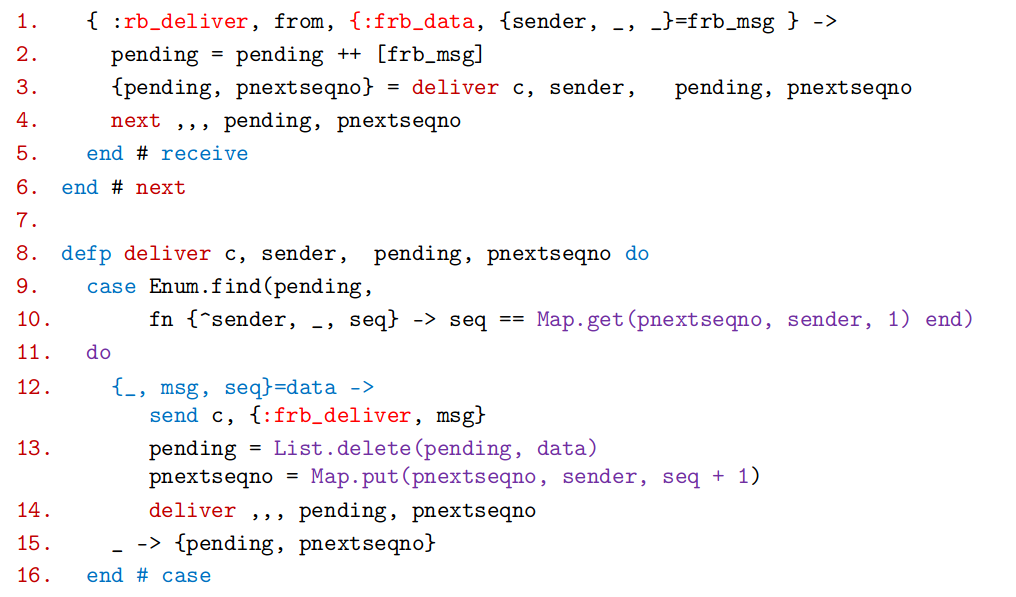
\includegraphics[scale=0.3]{frbcode2}
\end{figure}

\subsection{Causal Order RB (CRB)}
\begin{figure}[htb!]
  \centering
  \caption{CRB component.}
  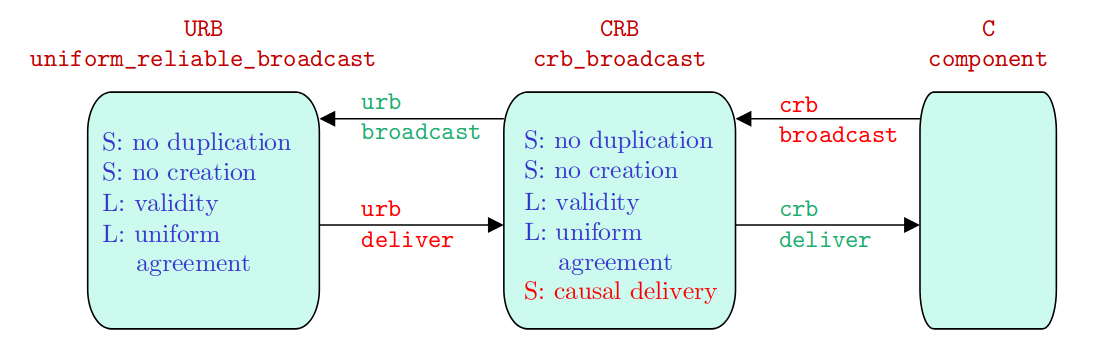
\includegraphics[scale=0.3]{crb}
\end{figure}

The \textbf{causal order relation} $m1 \rightarrow m2$ states that $m1$ may have caused $m2$ if the following apply:
\begin{itemize}
  \item \textbf{FIFO order} - Alice broadcasts $m1$, and later $m2$.
  \item \textbf{Local order} - Alice delivers $m1$, and later broadcasts $m2$.
  \item \textbf{Transitivity} - if there is a message $m3$ such that $m1 \rightarrow m3$, and $m3 \rightarrow m2$.
\end{itemize}

The \textbf{causal delivery property} ensures that if any process delivers $m2$, it must have previously delivered every message $m1$ such that $m1 \rightarrow m2$, thus ensuring that ``cause-effect'' relations are respected.

We never delay \texttt{crb\_deliver}ing a message - if we receive $m2$ and $m1$ was in the past, then we deliver $m1$ then $m2$ in causal order.
If we then receive $m1$ again, we can safely discard it.
\begin{itemize}
  \item \textbf{No Duplication (S)}, \textbf{No Creation (S)}, \textbf{Validity (L)}, and \textbf{Uniform Agreement (L)} are derived from the URB.
  \item \textbf{Causal Delivery (S)} is ensured by every message carrying its causally past messages, and by forcing them to be delivered before the message.
\end{itemize}
Carrying the entirety of the message's past means the overall message size can grow very large - we can optimize by purging messages from \texttt{past}.

\begin{figure}[htb!]
  \centering
  \caption{CRB code, part 1.}
  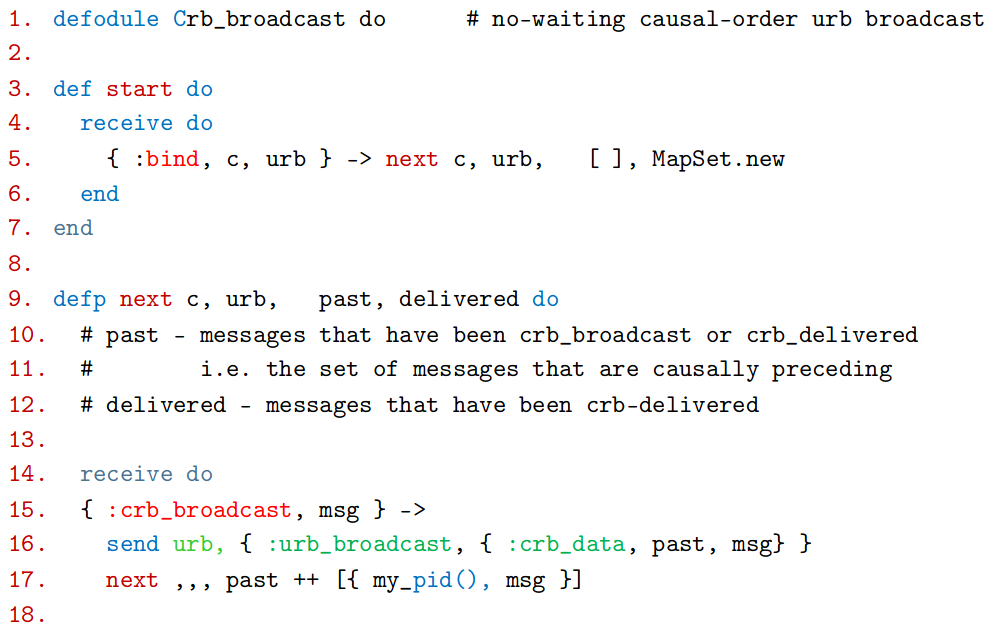
\includegraphics[scale=0.3]{crbcode1}
\end{figure}

\begin{figure}[htb!]
  \centering
  \caption{CRB code, part 2.}
  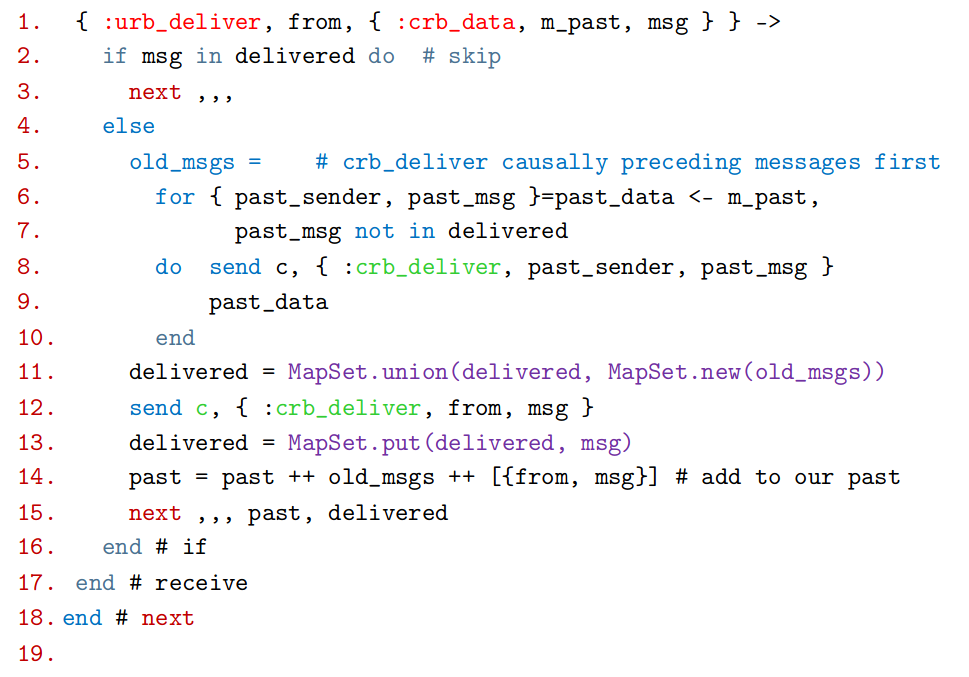
\includegraphics[scale=0.3]{crbcode2}
\end{figure}

\subsubsection{CRB with Vector Clocks}
We can use \textbf{vector clocks} to avoid storing past messages.
The vector clock (an array of sequence numbers) indicates the number of messages from each process that have been delivered.
Each process also maintains a count of the number of messages it has broadcast.

When a process broadcasts, it includes its vector clock with its own entry set to the broadcast's sequence number.
The receiving process, before delivering a message $M$, must compare the vector clock of the message with its own, the difference is the number of messages that must be delivered before $M$ - the process must defer delivering if necessary.

\begin{figure}[htb!]
  \centering
  \caption{CRB with vector clock code, part 1.}
  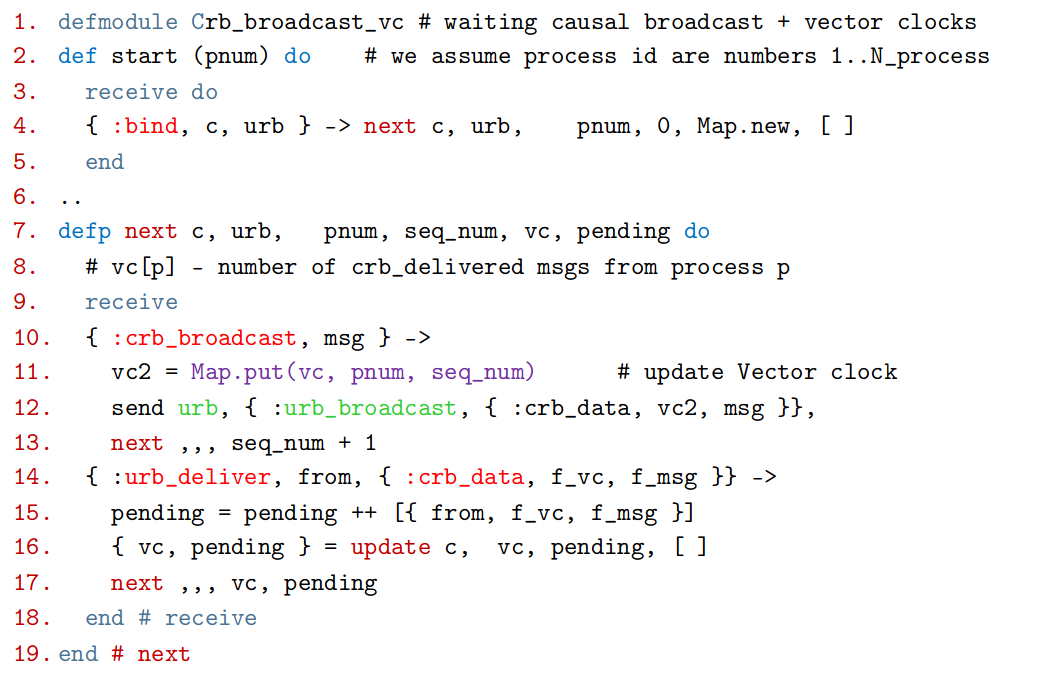
\includegraphics[scale=0.3]{vccode1}
\end{figure}

\begin{figure}[htb!]
  \centering
  \caption{CRB with vector clock code, part 2.}
  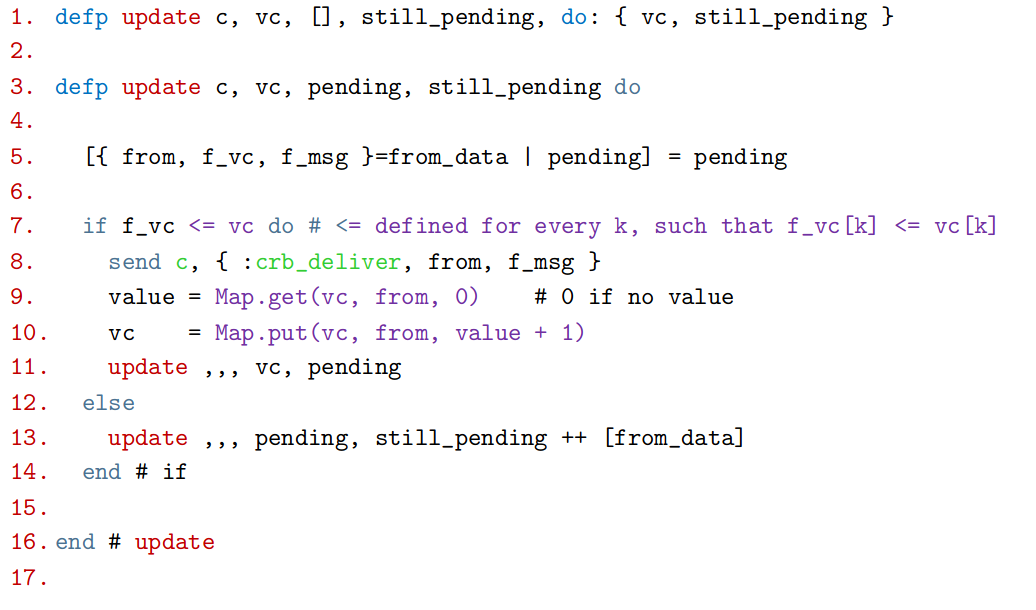
\includegraphics[scale=0.3]{vccode2}
\end{figure}

\subsection{Total Order Broadcast}
All processes must deliver all messages in the same order.
Causality or FIFO does not need to be respected but can be made to do so.

\subsubsection{Uniform Total Order Broadcast (TOURB)}
We require the 4 properties of URB, plus the following:
If $P$ is a correct process and delivers $M1$ without having delivered $M2$, no correct process delivers $M2$ before $M1$.

This is equivalent to the consensus problem - solving this problem solves the total order problem.
However, this problem cannot be solved in a completely asynchronous system.

\section{Consensus}
Consensus is how correct processes in a distributed system agree on a value.
Each process \textbf{proposes} a value, all processes must agree on (\textbf{decide} or \textbf{choose}) one of the proposed values.
Often these values are actions or commands to be carried out by a set of replicated servers.

Consensus can be used for total order broadcast, as processes must agree on message delivery order - and thus total order broadcast can be used for consensus.

In the \textit{non-blocking commit problem}, each process performs its own local computation and then the processes collectively either commit or abort their local computation.
Using consensus, each process proposes a \textit{yes} or a \textit{no} - if there is a \textit{no} proposal, then all local computations are aborted, otherwise all are committed.

More generally they can be used in any distributed system where processes have to agree on the \textbf{state of the application} before proceeding.

\subsection{Uniform Consensus}
\begin{itemize}
  \item \textbf{Validity (S)} - if a process decides on a value, then some process proposed it.
  \item \textbf{Integrity (S)} - a process decides one value at most.
  \item \textbf{Termination (L)} - each correct process eventually decides.
  \item \textbf{Uniform Agreement (S)} - no two processes decide different values.
\end{itemize}
Consensus does not specify which proposal is decided, only that the decision is one of the proposals.

With \textbf{regular consensus}, we replace uniform agreement with:
\begin{itemize}
  \item \textbf{Agreement (S)} - no two \textbf{correct} processes decide different values.
\end{itemize}

\subsection{Primary Backup}
Consider a simple algorithm with two servers, $S1$ and $S2$.
$S1$ is the leader and decides which requests to choose: if $S1$ chooses $r1$, it must tell $S2$.
We look into two cases after $S1$ chooses $r1$:
\begin{itemize}
  \item If $S2$ crashes before an \texttt{ack} is sent, $S1$ should continue and execute $r1$
  \item If $S1$ crashes after $r1$ is sent, $S2$ should continue and execute $r1$.
\end{itemize}
However, suppose $r1$ takes too long to reach $S2$ after being sent by $S1$.
Then $S2$ will execute $r2$ instead, thinking $S1$ has crashed.
$S1$ will execute $r1$ if \texttt{ack} takes too long to reach $S1$.
Then \textbf{consensus is violated}.

\subsection{FLP Impossibility Result}
Consensus cannot be solved in a purely asynchronous system where processes can crash.
This result applies even where:
\begin{itemize}
  \item Processes want to agree only on a single bit value.
  \item Message passing is reliable.
  \item At most 1 process crashes (even if there are thousands of correct processes).
\end{itemize}
In a purely asynchronous system, we cannot tell if a process has crashed or if it is slow to respond - there is no bound on the time taken to transmit messages.

\subsection{$\diamond$ Synchronous System}
In an eventually synchronous system (\textbf{$\diamond$ synchronous system}), messages take up to time $mT$ most of the time, but sometimes longer - how often they take longer is bounded but not known.
We can have consensus in a $\diamond$ synchronous system.

\subsubsection{Rotating Leaders}
Let us consider how we could use a $\diamond$ synchronous system.

\begin{itemize}
  \item Each round has a \textbf{leader}, we rotate between servers.
  \item The length of the round is set such that it is sufficient for servers to complete all the messages needed to make a choice.
  \item If messages take longer, we give the next server a chance to be leader and make the decision.
  \item We will eventually reach a round where the messages take $< mT$ and we can make a choice.
\end{itemize}

Suppose we only have two servers, $S1$ and $S2$.
If they do not hear from each other, they will keep swapping leadership forever.
We do not know the bound on the number of times messages will take longer than $mT$ but we do know that the system will be eventually synchronous and we want to tolerate crashes, but we cannot with only two servers as the other server may never respond quickly enough.

We can have consensus in a system with \textbf{$2f + 1$ servers in a $\diamond$ synchronous system}, if only up to $f$ servers crash.

\subsection{Paxos}
We now consider a basic example of a system with 3 servers: $S1$, $S2$, and $S3$.

Suppose $S1$ is the leader, and the rest witnesses:
\begin{itemize}
  \item $S1$ \textbf{consults} the other servers.
  \item The other servers reply with their \textbf{most recent value} and which \textbf{round} it was witnessed.
  \item $S1$ selects the \textbf{most recent value received}, and \textbf{proposes} it to the other servers.
  \item The other servers \textbf{accept} this, and send an acknowledgement back to $S1$.
  \item Finally, $S1$ sends the value selected as its \textbf{decision} to everyone, who then update their values.
\end{itemize}

\subsubsection{Crashes}
If any of the witnesses crash, then $S1$ can continue as they are expecting a message from the other witness.

If $S1$ crashes, then the witnesses will move the next round when the end of the round is reached, messages from earlier rounds are ignored, and the next leader $S2$ is selected.

\subsubsection{Safety and Liveness}
\begin{itemize}
  \item Safety - any value that is decided in a round must have been accepted by at least one other server, no other value that could be decided was in a higher round since it would have been selected and proposed.
  \item Liveness - we will eventually get to a round with sufficient time to complete the message exchanges within a round
\end{itemize}

\subsubsection{Round duration}
Rounds can have different durations, we can have longer rounds to ensure servers have enough time to complete their message exchange.

\subsubsection{Synchronous in Round 1}
Although Paxos is designed for $\diamond$ synchronous systems, it is very efficient if the system is synchronous from the start.
This requires that messages take less than $mT$, which is often very easy to do.

Therefore $S1$ will achieve consensus in the first round - furthermore, there is no need for consulting since there are no previous values, fast.

\subsubsection{Desynchronized Rounds}
The servers do not need be synchronized, they can rely solely on local clocks and move to the next round based on it - older rounds get ignored and slower servers are asked to catch up.

\subsection{Lamport's Basic Paxos}
Each Paxos component has 3 sub-components:
\begin{itemize}
  \item \textbf{Proposers} - \textbf{propose values} that they would like to be decided by acceptors; values are decided if they are accepted by a majority of acceptors.
  \item \textbf{Acceptors} - conditionally accept values from proposers.
  \item \textbf{Learners} - learn what values have been accepted and process them.
\end{itemize}
Each instance of the Basic Paxos algorithm decides a single value and can have several rounds.
A successful round has two phases: a \textbf{Prepare-Promise} phase and an \textbf{Accept-Accepted} phase.
\subsubsection{Phase 1: Prepare-Promise}
\begin{itemize}
  \item \textbf{Proposer: PREPARE request message}:
    \begin{itemize}
      \item Increase its (globally unique) proposal number, $PN$.
      \item Ask Acceptors to make a promise not to accept proposals less than its $PN$.
    \end{itemize}
  \item \textbf{Acceptor: PROMISE reply message}:
    \begin{itemize}
      \item Responds with the highest proposal it has accepted, or $\varnothing$ if no proposal has been accepted.
      \item If the Proposer's $PN$ is lower than the $PN$ of a previously made promise, respond with a negative acknowledgement.
    \end{itemize}
\end{itemize}

\subsubsection{Phase 2: Accept-Accepted}
\begin{itemize}
  \item \textbf{Proposer: ACCEPT request message}:
    \begin{itemize}
      \item Waits until promises have been received from a majority of Acceptors.
      \item Asks Acceptors to accept value $V$ with proposal number $PN$ - only needs to ask Acceptors that replied.
      \item $V$ is either the value of the highest promise made by the acceptors, or the Proposer's  own value if no Acceptors have made a promise.
    \end{itemize}
  \item \textbf{Acceptor: ACCEPTED reply message}:
    \begin{itemize}
      \item Accepts proposed value $V$ only if it has not made a higher promise.
      \item Returns value of highest $PN$ accepted.
    \end{itemize}
  \item \textbf{Proposer}:
    \begin{itemize}
      \item Waits until accepted replies are received from a majority of Acceptors.
      \item Retries (with higher $PN$) if a higher value was accepted by an Acceptor.
    \end{itemize}
\end{itemize}

\section{Leader Election}
In a distributed system, we do not want all the processes to run an algorithm in order to conserve resources.
We can achieve this by selecting one process from the network as the leader.

\subsection{Models and Assumptions}
Our network is \textbf{synchronous} and modelled as a digraph: $G = (V, E)$, where $\lvert V \rvert$ is the number of processes, and $E$ are the communication channels between them.
Processes consist of an initial state, a set of states, message generation function, and state transisiton function.

The leader election process can be initiated by any process in the system.
Each process maintains two boolean variables:
\begin{itemize}
  \item \texttt{done} - set when the leader election process is over.
  \item \texttt{leadeflag} - set when the process knows it is the leader.
\end{itemize}

A basic case has the processes arranged in a ring, with unidirectional or bidirectional communication around the ring.
Each process has a unique identifier (UID).

\subsection{Properties}
\begin{itemize}
  \item \textbf{Safety} - at most one process is elected as the leader.
  \item \textbf{Liveness} - eventually all processes should know a leader has been elected, and at least one process is a leader.
\end{itemize}

\subsection{LeLann, Chang, and Roberts (LCR) Algorithm}
The ring is unidirectional and has an unknown number of processes.
The process with the largest UID ends up as the leader.

\begin{enumerate}
  \item Each process in the ring sends its UID to its clockwise neighbour.
  \item When the process receives the UID, it compares it to its own UID:
    \begin{itemize}
      \item If it is smaller, \textbf{discard}.
      \item If it is bigger, \textbf{pass it on}.
      \item If it is equal, \textbf{declare yourself as leader} and let others know.
    \end{itemize}
\end{enumerate}

\subsubsection{Complexity}
We consider two complexities:
\begin{itemize}
  \item \textbf{Time complexity} - total number of rounds taken.
  \item \textbf{Message complexity} - total number of messages sent.
\end{itemize}

For time complexity, the message goes around at most $n$ hops before coming back to the original sender so $O(n)$.

The best case message complexity (processes in order of UID) is $O(n)$, the worst case (processes in reverse order) is $O(n^2)$.
The average case is $O(n \log n)$.

\subsection{Hirschberg-Sinclair (HS) Algorithm}
The ring is birdirectional and has an unknown number of processes.
The process with the largest UID ends up as the leader.

We carry out elections on increasingly larger sets (neighbourhoods).

\begin{enumerate}
  \item Each process operates in rounds ($0, 1, 2, \dots$).
  \item In round $k$, a process sends a message with its UID to $2^k$ neighbours on \textbf{both sides}, it proceeds to round $k + 1$ only if \textbf{replies arrive from both directions} (it is the leader of the local neighbourhood).
  \item When a process receives an outbound UID (inbound messages always forwarded) from its neighbour, it compares it to its own UID:
    \begin{itemize}
      \item If it is smaller, \textbf{discard it}.
      \item If it is bigger, \textbf{pass it on} unless you are the last node of neighbourhood, otherwise reply to the previous node (return to the originating node).
      \item If it is equal, \textbf{declare yourself as leader} and let others know.
    \end{itemize}
\end{enumerate}
Here outbound/inbound refer to the relative direction to the current neighbourhood origin and its ends.

\subsubsection{Complexity}
The time for each phase is $k = 2 \cdot 2^k$, as there are $2^k$ steps outbound and $2^k$ inbound.
The total time taken for phases $0$ to $k$ is $2 \cdot (2^0 + 2^1 + \dots + 2^k)$.
The time taken for the penultimate phase is $2^{O(\log n)}= O(n)$, and the last phase is $n$.
Then the time complexity is $2 + 4 + 8 + \dots + O(n) + n = O(n)$.

In phase $k$, if a process $P_i$ is the leader, then within its neighbourhood of $2^{k - 1} + 1$ processes there is only one leader.
The total number of leaders in phase $k$ is $\left\lfloor \frac{n}{2^{k - 1} + 1} \right\rfloor$.
The messages send/received by each leader in phase $k$ is $4 \cdot 2^k$, $4$ as we consider both directions inbound and outbound, $2^k$ from neighbourhood distance.
Then the number of messages in phase $k$ is $4 \cdot 2^k \cdot \left\lfloor \frac{n}{2^{k-1}+1}\right\rfloor \leq 8 \cdot n$.
The number of phases before the leader is elected is at most $1 + \left\lceil \log n \right\rceil$.
The the total nuber of messages is at most $8 \cdot n \cdot (1 + \left\lceil \log n \right\rceil)$.
The message complexity is $O(n \log n)$.

\subsection{Non-Comparison-Based Algorithms}
Any comparison-based leader election algorithm for a ring with unknown size has a message complexity of $\Omega(n \log n)$.

Let us now consider non-comparison-based algorithms, where the ring is unidirectional and the process UIDs are positive integers which we can manipulate with arithmetic operations.

In general, the message complexity is $O(n)$, but the timing complexity is very high.

\subsubsection{TimeSlice Algorithm}
The number of processes ($n$) in the ring is known.
\begin{enumerate}
  \item Divide into phases $1,2,3, \dots$ with each consisting of $n$ rounds.
  \item Phase $k$ is devoted to a process with UID $k$, if available.
  \item If a process has UID $k$, then in phase $k$ it sends its UID to its neighbour, who forwards it on through the network.
  \item When it reaches process $k$ again $k$ is elected, the number of messages is the number of nodes traversed ($n$).
\end{enumerate}
The process with the lowest UID ($UID_{min}$) is the leader.

The time complexity is $O(n \cdot UID_{min})$ (unbounded).

\subsubsection{VariableSpeeds Algorithm}
The number of processes in the ring is not known.
\begin{enumerate}
  \item Each process initiates a message with its UID and forwards it around the ring at the rate of 1 hop every $2^{UID}$ rounds - each process waits $2^{UID}$ rounds after receiving the message before forwarding it.
  \item If a process sees a message UID larger than the smallest UID it has seen so far, the message is discarded.
  \item The leader is the process whose message returns back to it, the message has travelled $n$ hops.
\end{enumerate}
The process with the lowest UID ($UID_{min}$) is the leader.

The time complexity is $O(n \cdot 2^{UID_{min}})$ (unbounded).

\subsection{FloodMax}
We relax the assumption that processes are arranged in a ring into a network of processes in a strongly connected digraph.

The diameter (or an upper bound on it) of the network is known, i.e.\ the longest distance between two nodes in the system.
The process with the largest UID ends up as the leader.

We wish to flood the network to propagate the UIDs.

Consider a process P with UID, $UID_P$:
\begin{enumerate}
  \item Keep track of the maximum UID seen so far ($UID_{max}$), initially $UID_P$.
  \item During each round, send $UID_{max}$ to all your outgoing channels.
  \item Repeat until the number of rounds is equal to the network diameter.
  \item If $UID_{max} = UID_P$, elect yourself as the leader.
\end{enumerate}
This is similar to LCR, but requires knowledge of the network.

\subsubsection{Complexity}
The time complexity is directly related to the diameter as the algorithm stops after $diameter$ rounds.

The message complexity is $\text{diameter } \multiply \text{ number of directed edges}$, as a message is sent along every directed edge.

\subsubsection{Optimisations}
\begin{itemize}
  \item Do not resend $UID_{max}$ to your neighbours every round, unless it changes (\textit{OptFloodMax}).
  \item If the new $UID_{max}$ was from a bidirectional neighbour, do not resend this along the same link during the next round.
\end{itemize}

\subsection{SyncBFS}
We require a method of calculating the diameter of the network -  we can build a spanning tree.

We assume that the network of processes is a strongly connected digraph, the number of processes is unknown, the diameter is unknown, each process has a UID.

A distinguished source node initiates the process:
\begin{enumerate}
  \item Initially the distinguished source process $P_0$ is marked.
  \item $P_0$ sends out a \textit{search} message to all its outgoing neighbours.
  \item During any round, if an unmarked process receives a \textit{search} message, it marks itself and chooses one of the processes from which it received this message as its parent.
  \item In the next round, that process sends a \textit{search} message to all its outgoing neighbours.
\end{enumerate}

\subsubsection{Complexity}
The time complexity is related to the diameter of the network.

The message complexity is $\lvert E \rvert$ since a \textit{search} message is sent once along each directed edge.

\subsubsection{Extensions}
It can be useful to know not only the parent processes but also the child processes.
This is easy with bidirectional links but requires indirect routes with unidirectional links (perhaps using another \textit{SyncBFS} execution).

\subsubsection{Convergecast}
Extend the previous idea to the whole network to allow the source node $P_0$ to detect termination of the algorithm - \textit{fan in} information from the leaves to the source node.

Each process sends notification of completion to its parent when:
\begin{itemize}
  \item It has received responses to all its search messages (knows its children).
  \item It has received notification of completion from all its children.
\end{itemize}

Termination is detected when $P_0$ receives replies from all its outgoing neighbours - this has the same issues with regards to unidirectional communication links.

\subsubsection{Applications}
\begin{itemize}
  \item \textbf{Broadcast communication} - add information onto the \textit{search} request, eventually all processes in the network will receive it.
  \item \textbf{Global computation} - perform accumulation using \textit{convergecast}.
  \item \textbf{Leader election} - all nodes run \textit{SyncBFS} in parallel and search for $UID_{max}$ using global computation on their own trees.
  \item \textbf{Diameter calculation} - all nodes run \textit{SyncBFS} in parallel and use  \textit{convergecast} to find diameter of each tree, then use \textit{convergecast} to find the maximum diameter.
\end{itemize}

\subsection{Asynchronous Networks}
In asynchronous networks, there is no notion of time so no bound on communication and execution time, nor any clock synchronisation (no rounds).

\section{Group Membership}
Group membership provides consistent and accurate information about which processes have crashed and which are correct, enabling dynamic changes in the list of processes that form the distributed system.

Better coordinated failures means potentially faster and simpler algorithms.

\subsection{Specification}
We consider that changes to the group occur only as a result of process crashes.

The \textbf{group} is the set of processes that participate in the system, a \textbf{view} is the current membership of the group.

We start with $V_0 = (0, \pi)$, where $0$ is the view identifier, and $\pi$ is the complete set of processes in the system.
Over time the system evolves with multiple views $V_n = (id, M)$.

\subsection{Properties}
\begin{itemize}
  \item \textbf{Monotonicity} - all correct processes install multiple views in a sequence  with monotonically increasing view identifiers.
  \item \textbf{Uniform Agreement} - two processes installing views with the same identifier will have the view containing the same set of processes as its members.
  \item \textbf{Completeness} - if a process $p$ crashes, then eventually every correct process will install a view which does not have $p$ as its member.
  \item \textbf{Accuracy} - if a process installs a new view which does not contain a process $p$, then $p$ must have crashed.
\end{itemize}

\subsection{Consensus-Based Group Membership}
We first assume that there is uniform consensus and perfect failure-detectors.
The algorithm is then:
\begin{enumerate}
  \item During initialisation, each process installs a view which includes all processes in the system.
  \item If a process is detected to have crashed, invoke uniform consensus.
  \item After consensus has been agreed, install the new view.
\end{enumerate}

\subsubsection{Correctness}
\begin{itemize}
  \item \textbf{Monotonicity} - a process initiates the formation of a new view (with a higher id) only when its current set is a subset of the current view membership.
  \item \textbf{Uniform Agreement} - follows from the unfirom agreement property of the underlying uniform consensus abstraction.
  \item \textbf{Completeness} - follows from the strong completeness property of the perfect failure-detector abstraction:
    \begin{itemize}
      \item If $p$ is detected as crashed then there will be a consensus instance in which every proposal will not include $p$.
      \item By the validity property of consensus, processes will eventually install a view that does not contain $p$.
    \end{itemize}
  \item \textbf{Accuracy} - if during consensus a process proposes a set of processes that did not include one of the processes, then that process must have been detected to have crashed (as a result of the perfect failure-detector).
\end{itemize}

At most \textbf{one consensus step} is needed for each process crash.

\subsection{View-Synchronous Communication}
Integrates reliable broadcast with group membership by providing an abstraction that gives  the illusion that failures are synchronized and appear to happen atomically with respect to the delivered messages - order the installation of views with respect to the message flow.

\end{document}

